\documentclass[12pt, french]{article}

\usepackage{fancyhdr, fancybox, lastpage,mhchem, mathrsfs, tikz}
\usepackage[most]{tcolorbox}
\usepackage[a4paper, margin={0.3in, .75in}]{geometry}
\usepackage{wrapfig}
\pagestyle{fancy}
\renewcommand\headrulewidth{1pt}
\renewcommand\footrulewidth{1pt}
\fancyhf{}
\rhead{ \em{Zakaria Haouzan}}
\lhead[C]{\em{2ème année baccalauréat Sciences Physiques}}
\chead[C]{}
\rfoot[C]{}
\lfoot[R]{}
\cfoot[]{\em{Page \thepage / \pageref{LastPage}}}


\newtcolorbox{Box2}[2][
enhanced, 
    breakable,
]{
                lower separated=false,
                colback=white,
colframe=white!20!black,fonttitle=\bfseries,
colbacktitle=white!30!gray,
coltitle=black,
enhanced,
attach boxed title to top left={yshift=-0.1in,xshift=0.15in},
title=#2,#1}


\begin{document}
\begin{center}
   \shadowbox {\bf{Lois de newton}
 }

\end{center}

\vspace{-0.2cm}
%%_________________________Exercice ! :"_________________________Exercice
   \begin{Box2}{Exercice 1 : Cas du mouvement sur plan horizontal sans frottement : }
  %\begin{center}
	  %\vspace{-0.6cm}
	%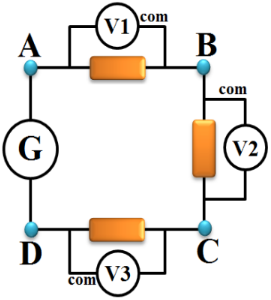
\includegraphics[width=0.42\textwidth]{./ex00.png}
  %\end{center}
%\end{wrapfigure}

 
% Required package
 
 
 
\begin{wrapfigure}{r}{0.27\textwidth}
	\vspace{-0.6cm}
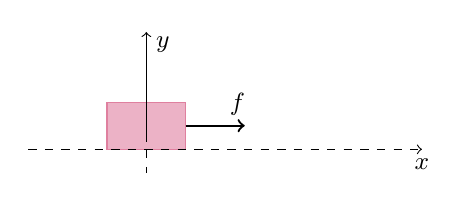
\begin{tikzpicture} [font = \small]
 
% triangle:
	\coordinate [pos=.45] (M); 
 
% angles:
%\draw [draw = orange] (O) ++(.8,0) arc (0:\ang:0.8) 
    %node [pos=.4, left] {$\theta$};
%\draw [draw = orange] (B) rectangle ++(-0.3,0.3);
 
%\begin{scope} [-latex,rotate=\ang]
 
% Object (rectangle)
\draw [fill = purple!30,
    draw = purple!50] (0,0) rectangle ++ (1,.6);
 
% Weight Force and its projections
\draw [dashed] (0,0) ++ (.5,.2) coordinate (MM) -- ++ (0,-.5)
node [very near end, right] { };
 
\draw [dashed, ->]  ++ (-1,0) -- (4,0) node [below] { $x$} ;
 

% Normal Force
\draw [->] (MM) -- ++ (0,1.29)
node [very near end, right] {$y$};
 
% Frictional Force
\draw [->, thick] (1,.3) -- ++ (0.75,0)
    node [very near end, above] {$f$};
 
%\end{scope}
 
\end{tikzpicture} 

\end{wrapfigure}
On considère un corps solide S en mouvement sur un plan horizontal sans frottement sous l'action d'une force constante $\vec{F}$
comme l'indique la figure suivante:

On donne : la masse du corps : $m=500g$ l’accélération de pesanteur $g=10 m/s^2$ et $F=2N$.
\begin{enumerate}
	\item  En appliquant la deuxième loi de Newton déterminer l'accélération du corps S.
	\item  Sachant que le corps part du point d'abscisse $x =-5cm$ à $t=0$ avec une vitesse égale à $3m/s$ , donner l'équation horaire de son
mouvement.
\end{enumerate}
   \end{Box2}


%%_________________________Exercice !2 :"_________________________Exercice
\begin{Box2}{Exercice 2 :Cas du mouvement sur plan horizontal avec frottement : }
   % \begin{wrapfigure}[6]{r}{0.32\textwidth}
  %\begin{center}
	  %\vspace{-0.6cm}
	%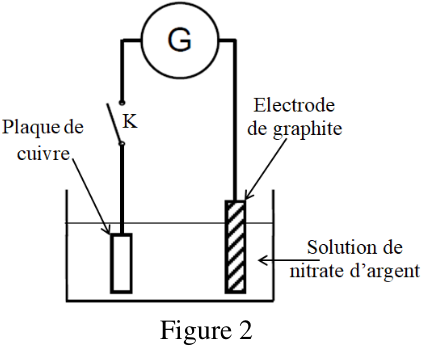
\includegraphics[width=0.32\textwidth]{./ex_01.png}
  %\end{center}
%\end{wrapfigure}

	\begin{wrapfigure}[4]{r}{0.27\textwidth}
	\vspace{-0.6cm}
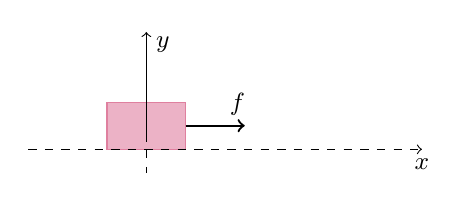
\begin{tikzpicture} [font = \small]
% triangle:
	\coordinate [pos=.45] (M);  
% angles:
% Object (rectangle)
\draw [fill = purple!30,
    draw = purple!50] (0,0) rectangle ++ (1,.6);
% Weight Force and its projections
\draw [dashed] (0,0) ++ (.5,.2) coordinate (MM) -- ++ (0,-.5)
node [very near end, right] { };
\draw [dashed, ->]  ++ (-1,0) -- (4,0) node [below] { $x$} ;
% Normal Force
\draw [->] (MM) -- ++ (0,1.29)
node [very near end, right] {$y$};
% Frictional Force
\draw [->, thick] (1,.3) -- ++ (0.75,0)
    node [very near end, above] {$f$};

\end{tikzpicture} 
\end{wrapfigure}


On considère le corps solide S précédent en mouvement sur un plan horizontal(avec frottement) sous l'action d'une force $\vec{F}$
et son accéleration devient $6m/s^2$

On donne : la masse du corps : $m=500g$  et $g=10m/s^2$ $F=5N$.
\begin{enumerate}
	\item En appliquant la deuxième loi de Newton déterminer l'intensité de la réaction du plan $\vec{R}$.
	\item Déterminer le coefficient de frottement puis en déduire la valeur de l'angle de frottement.
\item Sachant que le corps part du point d'abscisse $x=0$ à $t=0$ avec une vitesse égale à $1m/s$ , donner l'équation horaire de son mouvement.
\end{enumerate}

\end{Box2}

\begin{Box2}{Exercice 3 :Cas du mouvement sur plan incliné sans frottement : }


\begin{wrapfigure}[3]{r}{0.33\textwidth}
	\vspace{-0.8cm}
	\newcommand{\ang}{30}
 
\begin{tikzpicture} [font = \small]
 
% triangle:
\draw [draw = orange, fill = orange!15] (0,0) coordinate (O) -- (\ang:6)
    coordinate [pos=.45] (M) |- coordinate (B) (O);
 
% angles:
\draw [draw = orange] (O) ++(.8,0) arc (0:\ang:0.8) 
    node [pos=.4, left] {$\alpha$};
\draw [draw = orange] (B) rectangle ++(-0.3,0.3);
 
\begin{scope} [-latex,rotate=\ang]
 
% Object (rectangle)
\draw [fill = purple!30,
    draw = purple!50] (M) rectangle ++ (1,.6);
 
% Weight Force and its projections

    %node [very near end, right] {$mg\cos{\theta}$};
 
	\draw [dashed] (5,0) -- ++ (-6,0) node[above] {$B$}
    node [very near end, left] {$x$};
 
%\draw (MM) -- ++ (-\ang-90:1.5)
    %node [very near end,below left ] {$mg$};
 
% Normal Force
	\draw[dashed] (5,0) node[right]  {A}-- ++ (0,1.4)
node [very near end, right] {$y$};
 
% Frictional Force
%\draw (MM) -- ++ (0.75,0)
    %node [very near end, above] {$f$};
 
\end{scope}
 
\end{tikzpicture}
\end{wrapfigure}
	On libère un corps S de masse m=80kg sur un plan incliné d'un angle $\alpha =30^{\circ}$
par rapport à l'horizontale et il glisse sans
frottement vers le bas (voir figure).


\begin{enumerate}
	\item  En appliquant la deuxième loi de Newton déterminer les coordonnées 

		du vecteur accélération dans le repère $(O,x,y)$ associé
à un référentiel \\terrestre supposé Galiléen. puis déterminer l'intensité de la réaction \\du plan incliné.
\item  Sachant que le corps S part à l'instant $t=0$ du point A avec une vitesse $v_A= 5m/s$ (A est confondu avec l'origine O du repère
d'espace).
\begin{enumerate}
	\item donner l'équation horaire du mouvement de S selon l'axes(o,x) puis l'équation de sa vitesse .
	\item Déterminer sa vitesse au point B (on donne $AB=2m$ et $g=10m/s^2$
	\end{enumerate}
\end{enumerate}



\end{Box2}
	%\vspace{-0.8cm}


\begin{Box2}{Exercice 4 :Cas du mouvement sur plan incliné avec frottement : }


\begin{wrapfigure}[3]{r}{0.33\textwidth}
	\vspace{-0.8cm}
	\newcommand{\ang}{30}
 
\begin{tikzpicture} [font = \small]
 
% triangle:
\draw [draw = orange, fill = orange!15] (0,0) coordinate (O) -- (\ang:6)
    coordinate [pos=.45] (M) |- coordinate (B) (O);
 
% angles:
\draw [draw = orange] (O) ++(.8,0) arc (0:\ang:0.8) 
    node [pos=.4, left] {$\alpha$};
\draw [draw = orange] (B) rectangle ++(-0.3,0.3);
 
\begin{scope} [-latex,rotate=\ang]
 
% Object (rectangle)
\draw [fill = purple!30,
    draw = purple!50] (M) rectangle ++ (1,.6);
 
% Weight Force and its projections

    %node [very near end, right] {$mg\cos{\theta}$};
 
	\draw [dashed] (5,0) -- ++ (-6,0) node[above] {$B$}
    node [very near end, left] {$x$};
 
%\draw (MM) -- ++ (-\ang-90:1.5)
    %node [very near end,below left ] {$mg$};
 
% Normal Force
	\draw[dashed] (5,0) node[right]  {A}-- ++ (0,1.4)
node [very near end, right] {$y$};
 
% Frictional Force
\draw (3.7,.3) -- ++ (0.75,0)
	node [very near end, above] {$f$};
 
\end{scope}
 
\end{tikzpicture}
\end{wrapfigure}
On tire un corps S de masse m=100kg sur un plan incliné d'un angle $\alpha=10^{\circ}$
par rapport à l'horizontale par un câble et il glisse vers le haut(voir figure).


Sachant que le contact se fait avec frottement et que le coefficient de frottement 

est k=0,25 et son accélération selon l'axe $Ox$
est $a_x=2m/s^2$ .

\begin{enumerate}
	\item  En appliquant la deuxième loi de Newton déterminer les composantes de la réaction $\vec{R}$
du plan.

\item  Déterminer l'intensité de la force de traction $\vec{F}$
exercée par le câble sur le corps S. on donne $g=10m/s^2$
\end{enumerate}
\end{Box2}




\begin{Box2}{Exercice 5 : Cas d'un mouvement curviligne (utilisation du repère de Frenet) : }

%\begin{wrapfigure}[3]{r}{0.33\textwidth}
	%\vspace{-0.8cm}
	\newcommand{\ang}{-30}
 
Un corps solide S de masse m=100g se déplace sur un rail ABCD contenant trois portions:
\begin{center}
\begin{tikzpicture} [font = \small]
 
% triangle:
	\draw [draw = orange, fill = orange!15] (0,0) coordinate (O) node [right] {A} -- (\ang:6)node[below] {B} coordinate (C) coordinate [pos=.45] (M) -|  coordinate (B) (O);
% angles:
	\draw [draw = orange] (M) -- ++(\ang:2) arc (0:\ang+80:-0.8) 
    node [pos=.4, left] {$\alpha$};
\draw [draw = orange] (B) rectangle ++(0.3,0.3);

\draw (C) -- ++(0: 7) node[above] {C}  arc (90:15:2); 

%boule
\draw (M)++(0,.3) circle (7pt);
\fill[gray] (M) ++(0,.3)circle (7pt);

\draw[dashed] (C) -- ++(0: 7) -- ++(-90: 1.5) node[left] {O} node[pos=.6,above right]{$\theta$} -- ++(0:2) node[right] {D}; 
\draw[dashed] (C) -- ++(0: 7) -- ++(-90: 1.5) --++(60:1.5) ;
\end{tikzpicture}
\end{center}
\begin{itemize}
	\item La portion AB est inclinée d'un angle sur laquelle le mouvement se fait sans frottement . $AB=90cm$ et $\alpha=30^{\circ}$.

	\item  La portion $BC$ est rectiligne .$BC=2m$
	\item  La portion $CD$ est circulaire de centre O et de rayon r sur laquelle le mouvement se fait sans frottement.
\end{itemize}

\begin{enumerate}
	\item Le corps S part du point A sans vitesse initiale.
		\begin{enumerate}
			\item Déterminer l'accélération du corps S sur la portion AB puis en déduire la nature du mouvement . on prend $g=10m/s^2$
			\item Déterminer la vitesse $v_B$ du corps S au point B.
		\end{enumerate}
	\item   sachant qu'il y'a frottement et que la force de frottement est $f=0,225N$. Le corps S continue son mouvement sur le rail CD.
		\begin{enumerate}
			\item  En appliquant le théorème de l'énergie cinétique entre C et M , montrer que l'expression de la vitesse du mobile au point M s'écrit : $v=\sqrt{2.g.r(1-cos(\theta)}$
			\item Représenter au point M le repère de Frenet $(M,\vec{u},\vec{n})$
et les forces qui s'exercent sur le corps.
\item En appliquant la deuxième loi de Newton sur le corps S au point M et par projection sur la normale $(M,\vec{n})$ monter que l’intensité de la réaction exercée par le plan de contact sur S est : $R=m.g.(3.cos(\theta -2)$.
\item Sachant que le corps quitte le rail au point Mo repéré par l'angle $\theta_0$
.Déterminer la valeur de $\theta_0$
\end{enumerate}
\end{enumerate}



\end{Box2}


\begin{center}
   \Large{ \em{Exercices Supplémentaires}}
\end{center}

%\vspace{-0.8cm}

%%_________________________Exercice ! 3:"_________________________Exercice
\begin{Box2}{Exercice 6: La synthèse }
%\begin{wrapfigure}{r}{0.4\textwidth}
  %\begin{center}
	%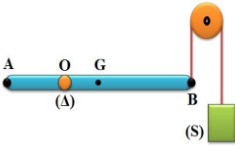
\includegraphics[width=0.4\textwidth]{./ex02.png}
  %\end{center}
%\end{wrapfigure}

Le ski sur la glace, est l’un des sports les plus répandus dans les régions montagnardes. Les pratiquants de ce
sport visent à réaliser des résultats positifs et battre des records.
Le but de cet exercice est d’étudier le mouvement d’un sportif, pratiquant le ski sur des trajectoires de glace
diverses.
 \begin{center}
	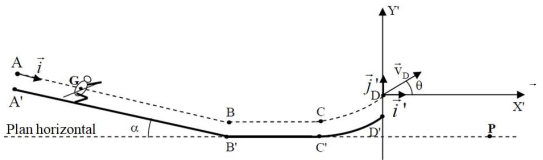
\includegraphics[width=0.6\textwidth]{./ex_06.png}
  \end{center}

Le circuit de ski représenté sur la figure ci-dessous, est constitué de trois parties :
\begin{itemize}
	\item Une partie A’B’ rectiligne de longueur  A’B’ = 82,7 m, inclinée d’un angle $\alpha$ = 14° par rapport au plan horizontal ;
	\item  Une partie B’C’ rectiligne horizontale, de longueur L = 100 m ;
	\item  Une partie C’D’ circulaire
\end{itemize}

On modélise le sportif et ses accessoires par un solide (S) de masse $m = 65 Kg$, et de centre d’inertie G.
On prendra : $g = 10 m.s^{-2}$.

G passe au cours de son mouvement par les positions A, B, C et D représentées sur la figure, tel que :
A’B’ = AB et B’C’ = BC.

\section*{\underline{1. Etude du mouvement sur la partie A’B’ :}}
A l’instant $t = 0$, G part de A sans vitesse initiale, le solide (S) glisse ainsi sans frottements sur la
partie A’B’.

On repère la position de G, à un instant t, par l’abscisse x dans le repère $(A.\vec{i})$ , et on considère que $x_G$=0 à l’instant t = 0.

1.1- Par application de la deuxième loi de Newton, établir l’expression de l’accélération $a_G$ du
mouvement de G en fonction de g et $\alpha$.

1.2- Déterminer en justifiant votre réponse la nature du mouvement de G sur cette partie.

1.3- A l’aide des équations horaires du mouvement, trouver la valeur $v_B$ de la vitesse de G lors du
passage par la position B.

\section*{\underline{2- Etude du mouvement sur la partie B’C’ :}}

Le solide (S) poursuit son mouvement sur la partie B’C’, où il subit des frottements modélisés par une
force f constante, tangente à la trajectoire et de sens inverse à celui du mouvement.
On considère que la valeur de la vitesse de G au point B ne varie pas lors du passage du solide (S) du plan
incliné au plan horizontal.

Pour étudier le mouvement de G sur cette partie, on choisit, un repère horizontal
d’origine confondue avec le point B, et l’instant du passage de G en ce point comme nouvelle origine des
temps

2.1- En appliquant l a deuxième loi de Newton, déterminer la nature du mouvement de G sur le trajet BC.

2.2- Trouver l’expression de l’intensité f de la force de frottement en fonction de m, L, $v_B$ et $v_C$ vitesse
de G au point C, puis calculer f.

\textbf{On donne} : $v_C = 12 m.s^{-1}$.

\end{Box2}

%%_________________________Exercice 4 : _________________________Exercice
\begin{Box2}{Exercice 7 :Le ski }
   % \begin{wrapfigure}[12]{r}{0.5\textwidth}

%\end{wrapfigure}
Un skieur glisse sur une piste de ski, constituée par deux parties:

- Une partie A'B' rectiligne et inclinée d’un angle par rapport à l’horizontale.

- Une partie B'C' rectiligne et horizontale (voir figure).
  \begin{center}

	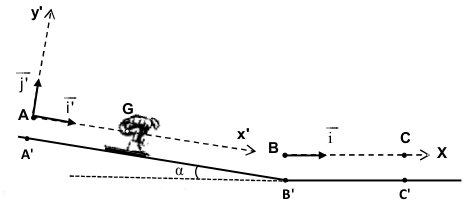
\includegraphics[width=0.5\textwidth]{./ex_07.png}
  \end{center}
\textbf{Données : }
\begin{itemize}
	\item $g = 9,8 m.s^{-2}$
	\item Masse totale du skieur et ses accessoires : $m = 65 kg$
	\item Angle d’inclinaison: $\alpha$ = 23°.
	\item On néglige la résistance de l’air.
\end{itemize}

\textbf{\underline{1- Etude du mouvement sur le plan incliné :}}

On étudie le mouvement du centre
d’inertie G du système (S), constitué par le skieur et ses 
accessoires, dans le repère $(A,\vec{i'}, \vec{j'})$ lié à un référentiel terrestre considéré galiléen.
Le système (S) se met en mouvement sans vitesse initiale depuis le point A , confondu avec G à
l’instant t=0, origine des dates.

Le mouvement de G se fait suivant la ligne de plus grande pente du plan incliné AB. ( AB = A'B' )
Le contact entre le plan incliné et le système (S) se fait avec frottements .La force de frottements
est constante d’intensité $f = 15 N$.


\textbf{1.1- }En appliquant la deuxième loi de Newton, montrer que l’équation différentielle vérifiée par la vitesse $v_G$ du mouvement de G s’écrit sous forme :$\frac{dv_G}{dt} = g.sin\alpha - \frac{f}{m}$

\textbf{1.2- }La solution de cette équation différentielle est de la forme : $v_G(t) = b.t + c$ . Déterminer les
valeurs de b et de c.

\textbf{1.3- }Déduire la valeur de $t_B$ , l’instant de passage du centre d’inertie G par la position B avec une
vitesse égale à $90 km.h^{-1}$.

\textbf{1.4- }Trouver l’intensité R de la force exercée par le plan incliné sur le système (S).


\textbf{2- Etude du mouvement sur le plan horizontal :}

Le système (S) continue son mouvement sur le plan horizontal B'C' pour s’arrêter à la position
C' . Le contact entre le plan horizontal et le système (S) se fait avec frottements . La force de
frottements est constante d’intensité f ' .

Le mouvement de G est étudié dans le repère horizontal $(B,\vec{i})$ lié à un référentiel terrestre considéré
galiléen.

Le centre d’inertie G passe par le point B avec une vitesse de $90 km.h^{-1}$ à un instant considéré
comme nouvelle origine des dates.

\textbf{2.1- }En appliquant la deuxième loi de Newton, trouver l’intensité $f'$ sachant que la composante
horizontale du vecteur accélération du mouvement de G est $a_x =-3m.s^{-2}$.

\textbf{2.2- }Déterminer $t_c$ , l’instant d’arrêt du système.

\textbf{2.3- }Déduire la distance $BC$ parcourue par G.
\end{Box2}
\begin{center} \emph{\textbf{MODERN problems require MODERN SOLUTION!!}}
\end{center}

%\vspace{-0.6cm}
%%%_________________________Exercice 5 : _________________________Exercice
%\begin{Box2}{Exercice 4 : }
   %% \begin{wrapfigure}[14]{r}{0.5\textwidth}
  %%\begin{center}
	  %%\vspace{-0.6cm}
	%%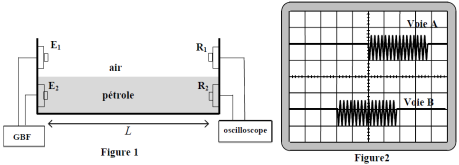
\includegraphics[width=0.5\textwidth]{./img/ex5.png}
  %%\end{center}
%%\end{wrapfigure}

%4

%\end{Box2}

%\begin{Box2}{Exercice 5 : }

%44
%\end{Box2}


%\begin{Box2}{Exercice 6 : }


	%\end{Box2}


%\begin{Box2}{Exercice 7 : }
%\end{Box2}
\end{document}
